
\documentclass[ms.tex]{subfiles}
\begin{document}
\renewcommand\theequation{\thesection\arabic{equation}}
\renewcommand\thefigure{\thesection\arabic{figure}}
\setcounter{equation}{0}
\setcounter{figure}{0}

\section{The Yield-Outflow Degeneracy}
\label{sec:yield_outflow_degeneracy}

\begin{figure*}
\centering
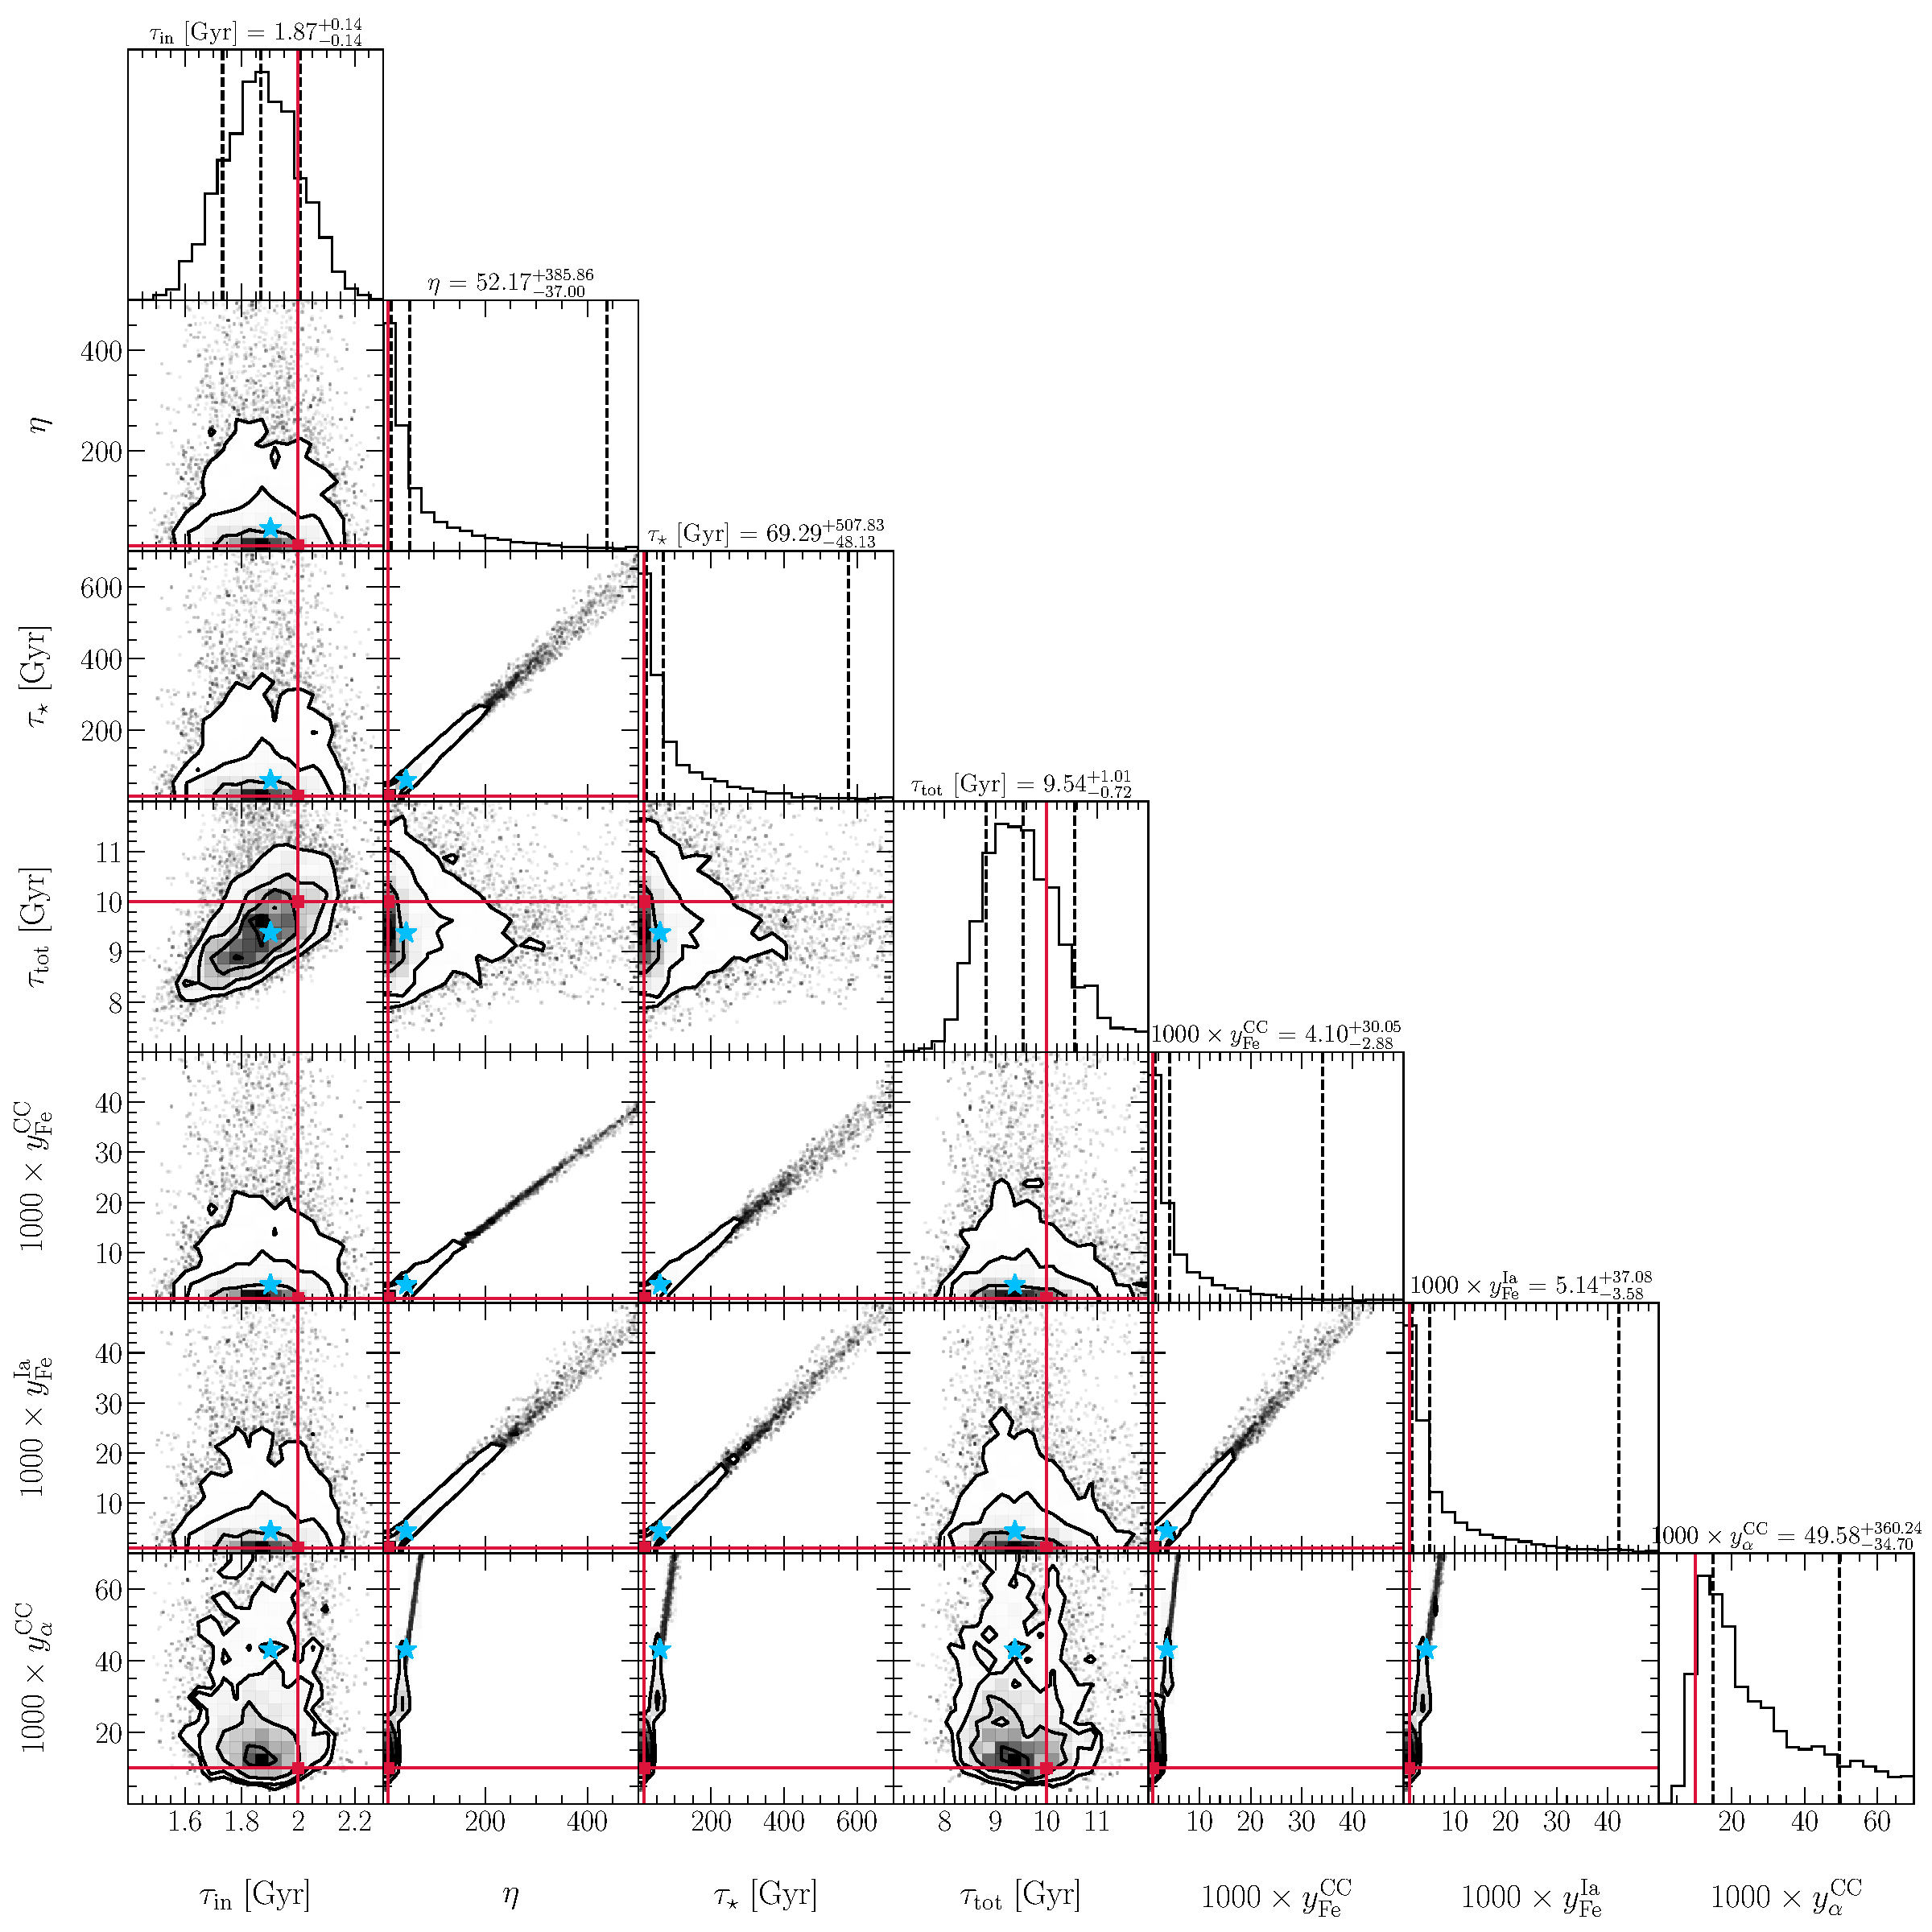
\includegraphics[scale = 0.4]{degeneracy_25k6.pdf}
\caption{
The same as Fig.~\ref{fig:fiducialmock}, but with the alpha element yield from
massive stars~\yacc~as an additional free parameter.
Motivated both by theoretical models of nucleosynthesis in massive stars and
the convenience for scaling up or down, we have adopted~$\yacc \equiv 0.01$
in this paper to set the scale of this degeneracy.
}
\label{fig:degeneracy}
\end{figure*}

\end{document}

